\documentclass[12pt]{article}
\usepackage[a4paper,top=2cm,bottom=2.5cm,left=1.5cm,right=1.5cm,marginparwidth=1.75cm]{geometry}
\usepackage[english]{babel}
\usepackage[utf8x]{inputenc}
\usepackage{listings}

\usepackage{float}
\usepackage{amsmath}
\usepackage[colorinlistoftodos]{todonotes}
\usepackage[colorlinks=true, allcolors=blue]{hyperref}
\usepackage{listings}
\usepackage{url}
\usepackage{graphicx}
\graphicspath{ {./images/} }
\DeclareGraphicsExtensions{.pdf,.jpg,.png}

\definecolor{Blue}{rgb}{0,0,0.5}
\definecolor{Green}{rgb}{0,0.75,0.0}
\definecolor{LightGray}{rgb}{0.6,0.6,0.6}
\definecolor{DarkGray}{rgb}{0.3,0.3,0.3}

\title{MN2: Assignment 2}
\author{Taras Yarema}
\date{\today}


\begin{document}
\maketitle

\section{C functions implemented}

\cite{MN2:1}

\section{Solving the system of equations using Newton's method}

\section{Plotting the curve}

\begin{figure}[h]
    \centering
    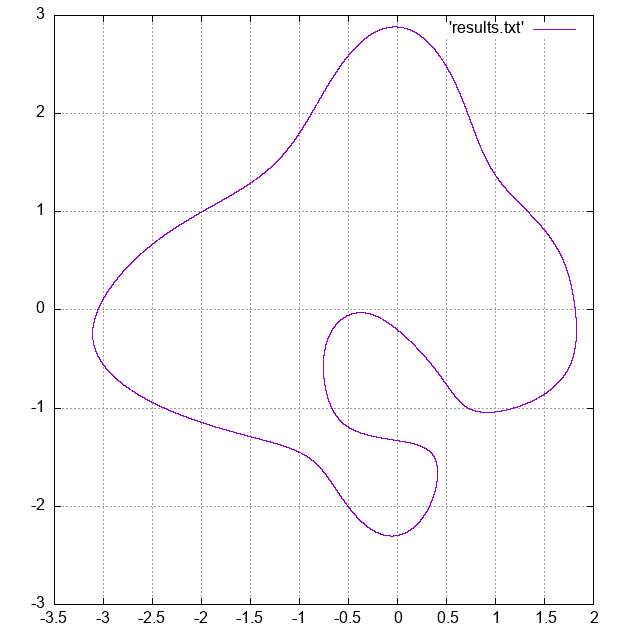
\includegraphics[width=0.5\textwidth]{got}
    \caption{Plot of the curve such that $f(C) = 0$, using \textbf{gnuplot}}
\end{figure}

\bibliographystyle{plain}
\bibliography{YaremaTaras}

\end{document}
